\chapter{無線センサネットワーク}
\begin{large}
\begin{quote}
本節では,最初に多次元データ管理Multidimensional Indexing(MI)の分野における関連研究を挙げる.次に,Contents Delivery Network(CDN)におけるコンテンツの特徴を利用したレプリケーションを行った研究を挙げる.最後に,センサデータを多次元データとして扱った研究を挙げる.
\end{quote}
\end{large}
\clearpage

\section{はじめに}
近年技術の発展によりセンサノードの低価格化,高性能化が進み,
それに伴い,ネットワークに繋がる物理センサが自動的に多様なデータをやり取りし,
それらを様々な形で活用する無線センサネットワークが普及してきている.
代表的なセンサノードとして,Iris MoteやMicaZ\cite{Hill:2002:MWP:623308.624560},
SunSPOTなどがある.

Iris Moteは図\ref{fig:iris_mote}のようなものであり,
アメリカのCrossbow Technology社が開発したセンサネットワーク用の無線端末である.
それに対して,MicaZはカリフォルニア大学バークレー校における
スマートダストプロジェクト\cite{Kahn:1999:NCC:313451.313558}によって開発された.
ハードウェア,OS,開発言語,シュミレータ,
ライブラリといったアプリケーション開発環境を提供しており,
アプリケーション開発が容易であるため,
現在センサネットワークの研究で多く使用されている.
図\ref{fig:micaz}にMicaZの写真を示す.
MicaZは小型なため,様々な場所に応用することができる.
SunSPOTは図\ref{fig:sunspot}のようなものであり,
サン・マイクロシステムズが開発したIEEE 802.15.4に準拠した無線センサーネットワークデバイスである.
SunSPOTとはSun Small Programmable Object Technologyの略称であり,
Javaで実装することができるため,初心者でも扱いやすいセンサデバイスとなっている.


\begin{figure}[htbp]
 \begin{minipage}{0.5\hsize} \begin{center}
     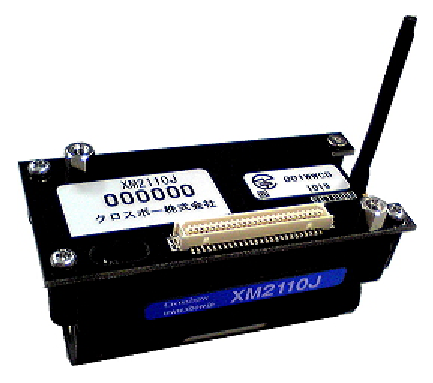
\includegraphics[width=40mm]{./images/iris_mote.eps}
    \end{center}
    \caption{Iris Mote}
    \label{fig:iris_mote}
 \end{minipage}
 \begin{minipage}{0.5\hsize}
    \begin{center}
     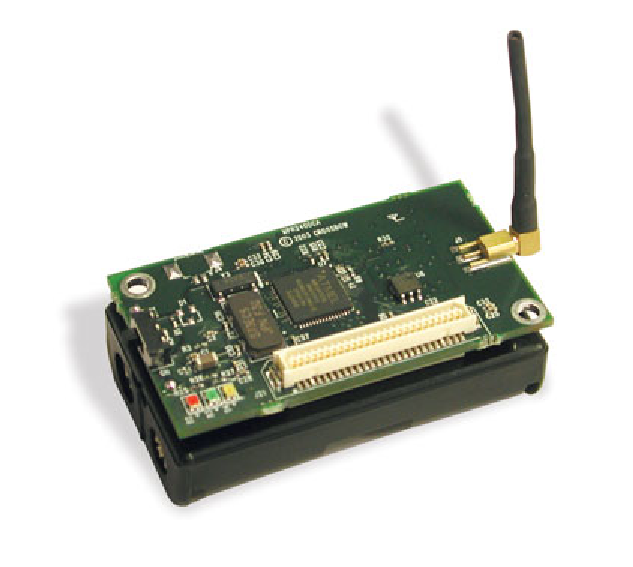
\includegraphics[width=45mm]{./images/micaz.eps}
    \end{center}
    \caption{MicaZ}
    \label{fig:micaz}
 \end{minipage}
\end{figure}

\begin{figure}[htbp]
 \begin{center}
  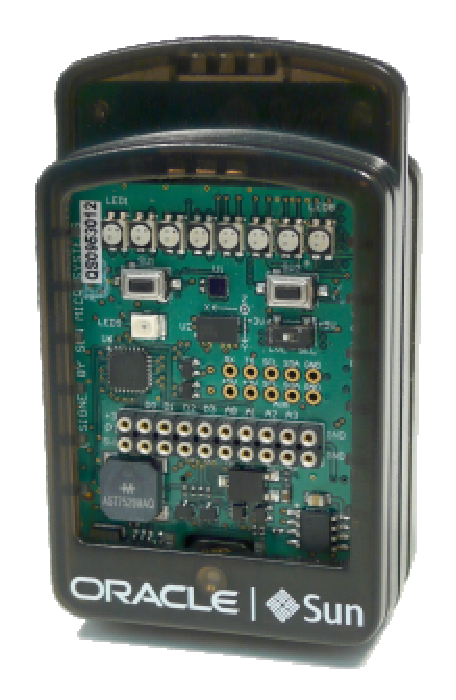
\includegraphics[width=25mm]{./images/sunspot.eps}
 \end{center}
 \caption{SunSPOT}
 \label{fig:sunspot}
\end{figure}





\section{環境モニタリング}

\subsubsection{森林火災検知}

\vspace{0.5em}センサノードが戦略的に,ランダムに,密集して森林に配置されれば,
火災が制御できなくなるほど広がる前に,
センサノードが正確な火の根源をユーザに知らせることが可能になる.
%Since sensor nodes may be strategically,randomly,and densely deployed in a forest,
%sensor nodes can relay the exact origin of the fire to the end users 
%before the fire is spread uncontrollable. 
数百万から構成されるセンサノードが
無線周波数を利用し,統合され,配置されることも可能である.
%Millions of sensor nodes can be deployed and integrated using radio frequencies/ optical systems. 
また,太陽電池などのような,利用可能なエネルギーを探索し,
効率的に活用する手法が備えられるかもしれない.
%Also,they may be equipped with effective power scavenging methods [12],
%such as solar cells,
%because the sensors may be left unattended for months and even years. 
センサノードは,分散しセンシングをするまたは木や岩のような障害に打ち勝つために,
それぞれが協調するだろう.
%The sensor nodes will collaborate with each other to perform distributed 
%sensing and overcome obstacles,
%such as trees and rocks,
%that block wired sensors’ line of sight.




\section{ターゲットトラッキング}
もし無線センサネットワークが適切に利用された場合,
軍用のアプリケーションにおける情報収集にて,
人間の力を必要とする機会が減少していき,
近い将来には,
センサデバイスが低価格で大量生産され,
実社会に高密度に備え付けられることが予測される.

\subsubsection{軍用監視システム}

\vspace{0.5em}監視任務において,
ターゲットとする敵の能力や位置に関する情報を
正確に入手することが何よりも重要であるが,
そのような任務には隊員の危険を伴うものが多い.
無線センサネットワークを利用することで,
リスクを最小限に抑えつつ,
敵の侵入に関する情報を的確に把握する研究が盛んに行われている.
図\ref{fig:surveillance_system}は軍用監視システムにおける概念図である.

\begin{figure}[htbp]
 \begin{center}
  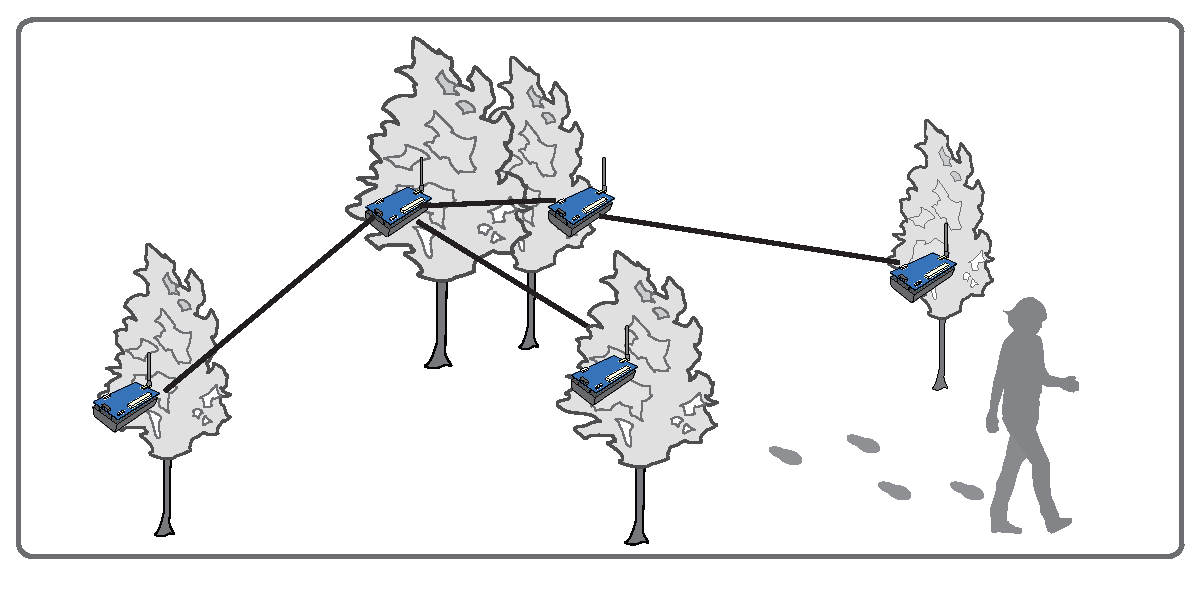
\includegraphics[width=100mm]{./images/surveillance_system.eps}
 \end{center}
 %\caption{イベント検知アプリケーション}
 %\caption{ターゲットトラッキングアプリケーション}
 \caption{軍用監視アプリケーションにおける概念図}
 \label{fig:surveillance_system}
\end{figure}


監視アプリケーションにおいて,
侵入者を検知し,その旨をシステムのゲートウェイノードに警告するタスクにより
中継されたデータは,
適時にゲートウェイまで届けられるべきである.
上記のような時間的制約を伴ったデータの配送が必要なアプリケーションを想定した場合,
オペレーティングシステムとして
リアルタイム処理を行うことが可能なものを選択することが多い.
無線センサネットワークにおけるオペレーティングシステムのリアルタイム性については,
\ref{sec:threads_model}において詳細に述べる.

監視システムアプリケーションを用いた任務は
数日から数ヶ月にかけて行われるものが一般的であり,
任務中の秘密保持の重大性や
任務が敵の管轄地域行われる場合もあることから,
%近づきにくさ
任務期間中に資源の制限されたセンサデバイスの手動による充電はできないことがほとんどである.
したがって任務期間中継続して使用するために,
監視システムにおけるアプリケーションでは
センサデバイスの寿命を向上させるような
省エネルギーな構成が必要とされる.

また軍用の監視システムにおいて,
デイバイスが発見され,
それに伴い迎撃されることを
未然に防ぐことは極めて重要である.
センサデバイスを小型化することにより,
デバイスの発見を物理的に困難にすることができるが,
もしセンサデバイスが監視をする際に活発に通信をする場合,
無線周波数が傍受されてしまう可能性が高い.
重要なイベントが発生したときを除いて,
通信を控えることが求められている.





\subsubsection{野生動物の生態調査}

\vspace{0.5em}



%\section{イベント検知アプリケーション}

\section{まとめ}
本章では,まず,公衆広域センサデータが多次元データであるということから,本研究の根幹を成す,Multidimensional Indexing(MI)という研究分野を紹介した.次に,Contents Delivery Network(CDN)という分散したデータセンターで多次元データを管理するネットワークという観点から捉え,センサデータにはCDNで扱われるような特殊性が存在しないことを述べた.最後に,公衆広域センサデータの分散管理手法を紹介し,センサデータの時間的特殊性が考慮されていないことに言及した.
